% slide 1
\begin{frame}[fragile]{Lektion 1}
\begin{figure}
    \centering
    \includegraphics[width=1\textwidth]{\thelogo.pdf}
    \caption*{Modellierung und Abstraktion durch Graphen}
\end{figure}
\end{frame}


% % slide 3
% \begin{frame}[fragile]{Computer Science Unplugged}
% \begin{itemize}[<+->]
%     \item Sie erhalten alle Unterlagen auf Papier.
%     \item Ich bitte Sie, Ihre Laptops und Smartphones zu verstauen.
% \end{itemize}
% \end{frame}


% slide 4 (IU)
% TODO: stimmen Lernziele noch. plastische operationalisierte Lernziele
% https://www.geeksforgeeks.org/applications-of-breadth-first-traversal/
\begin{frame}[fragile]{Thema und Lernziele}
\begin{itemize}[<+->]
    \item Thema: Grundlagen der Abstraktion und Modellierung mit Graphen
    \item Lernziele:
    \begin{itemize}
        \item Sie beschreiben Zugverbindungen und Computernetzwerke in der abstrakten Sprache der Informatik.
        \item Sie beschreiben drei Situationen aus Ihrem Alltag, die sich mathematisch elegant modellieren lassen.
        \item Sie erklären einer Kollegin (ohne Unterlagen) das historische Brückenproblem von Königsberg unter Verwendung der korrekten Begriffe.
        %\item Sie beschreiben mindestens drei Situationen aus Ihrem Alltag, die sich mathematisch elegant modellieren lassen.
        %\item Sie erklären warum eine von Ihnen gewählte Abstraktion ein gegebenes Problem korrekt beschreibt.
    \end{itemize}
\end{itemize}
\end{frame}


% slide 5 (IU)
% TODO: tabelle mit den 4 Spalten:
% Was, Wie, Wer, Dauer
\begin{frame}[fragile]{Ablauf der Lektion}
\begin{itemize}[<+->]
    \item zuerst: Einstieg von mir (Beamer)
    \item danach: Aufgabenblöcke (Sie sind gefragt!) unterbrochen durch kurze Besprechungen (gemeinsam)
\end{itemize}
% \begin{table}[H]
% \resizebox{1.0\textwidth}{!}{%
% \begin{tabular}{|l|l|l|l|}
% \hline
% \textbf{Was?}                                 & \textbf{Wer?} & \textbf{Wie} & \textbf{Zeit}    \\ \hline
% Einstieg                                      & gemeinsam     & Beamer       & 10 bis 15 Min.   \\ \hline
% 1. Aufgabenblock    & Sie           & Papier       & 5 Min.           \\ \hline
% kurze Besprechung der Aufgaben                & Sie           & Beamer       & 5 Min.           \\ \hline
% 2. Aufgabenblock & gemeinsam     & Papier       & 10 Min.          \\ \hline
% Beobachtung zum Brückenproblem                & gemeinsam     & Beamer       & 5 Min.           \\ \hline
% 3. Aufgabenblock                   & Sie           & Papier       & Rest der Lektion \\ \hline
% \end{tabular}%
% }%
% \end{table}
\end{frame}


% slide 6 (IU)
% TODO: meine positiven Erwartungen
% deutlich machen, wie ich das Thema finde
% Verbinden Sie das Thema mit solchen in den vergangenen oder künftigen Stunden
% Anerkennen Sie die Vorkenntnisse!
\begin{frame}[fragile]{Bemerkungen zu dem Thema} % <-- vielleicht kein Slide nötig!
\begin{itemize}[<+->]
    \item Für dieses Thema werden kaum Vorkenntnisse benötigt!
    % \item Spätestens in der zweiten Aufgabe werden Sie sehen, wie dieses Thema mit Ihren Webseiten zusammenhängt.
    \item Ich mag dieses Thema sehr, da es mir eine völlig neue Sichtweise auf diverse Alltagssituationen erlaubt.
    \item Ich bin überzeugt, dass die neuen Inhalte und Begriffe auch Ihre Denkweise prägen werden!
\end{itemize}
\end{frame}


% slide 7
\begin{frame}[fragile]{Eulers Besuch in Königsberg}
\begin{itemize}[<+->]
    \item Der berühmte Schweizer Mathematiker Leonhard Euler soll im Jahre 1736 die Stadt Königsberg besucht haben.
    \item Königsberg war damals die Hauptstadt der deutschen Provinz Ostpreussen.
    \item Seit dem Jahre 1946 gehört die Stadt zu Russland und wurde in \textit{Kaliningrad} unbenannt.
\end{itemize}
\end{frame}


% slide 8
\begin{frame}[fragile]{}
\begin{figure}
    \centering
    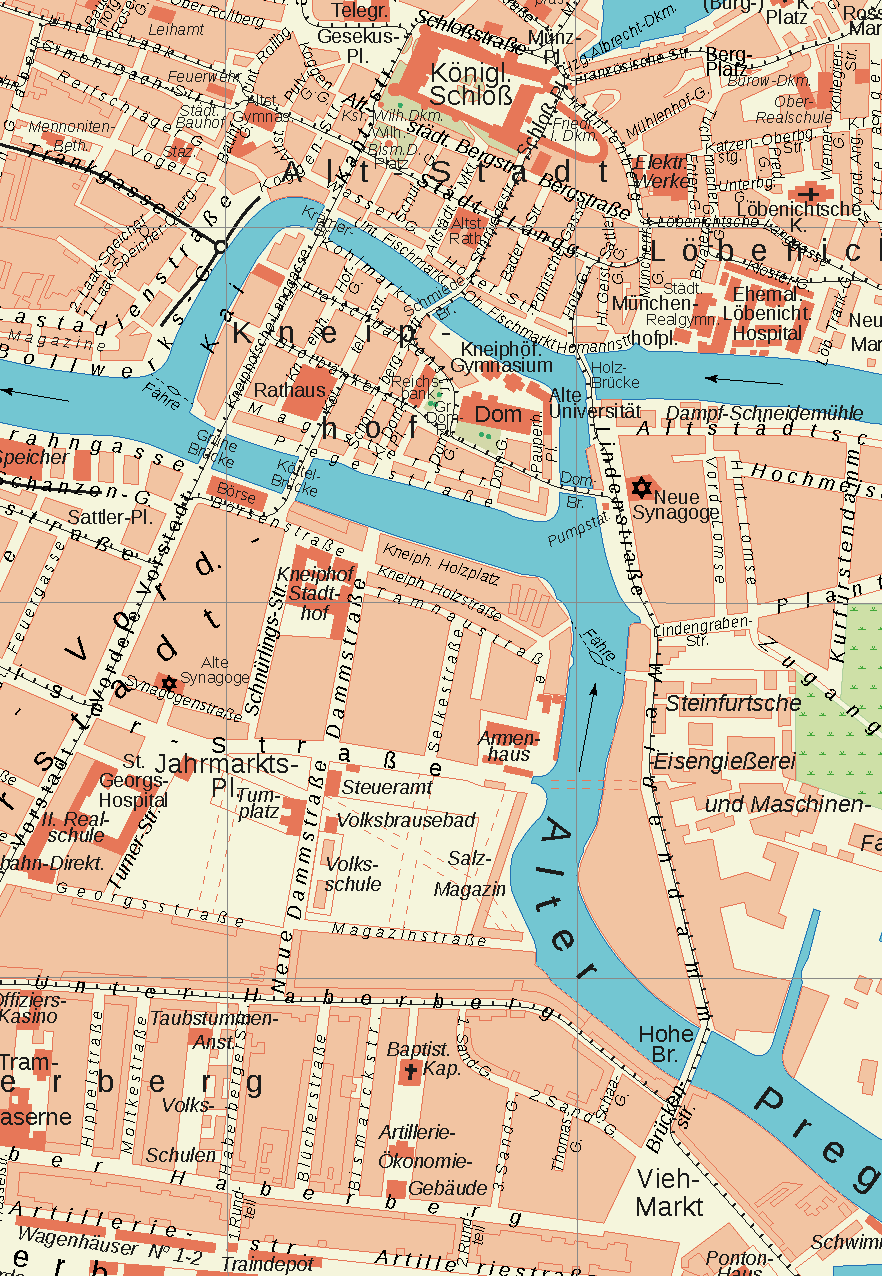
\includegraphics[width=0.5\textwidth]{Grundlagen_Info/02_Graphen/AbstraktionDurchGraphen/Figures/StadplanCrop.pdf}
\end{figure}
\end{frame}


% slide 9
\begin{frame}[fragile]{}
\begin{figure}
    \centering
    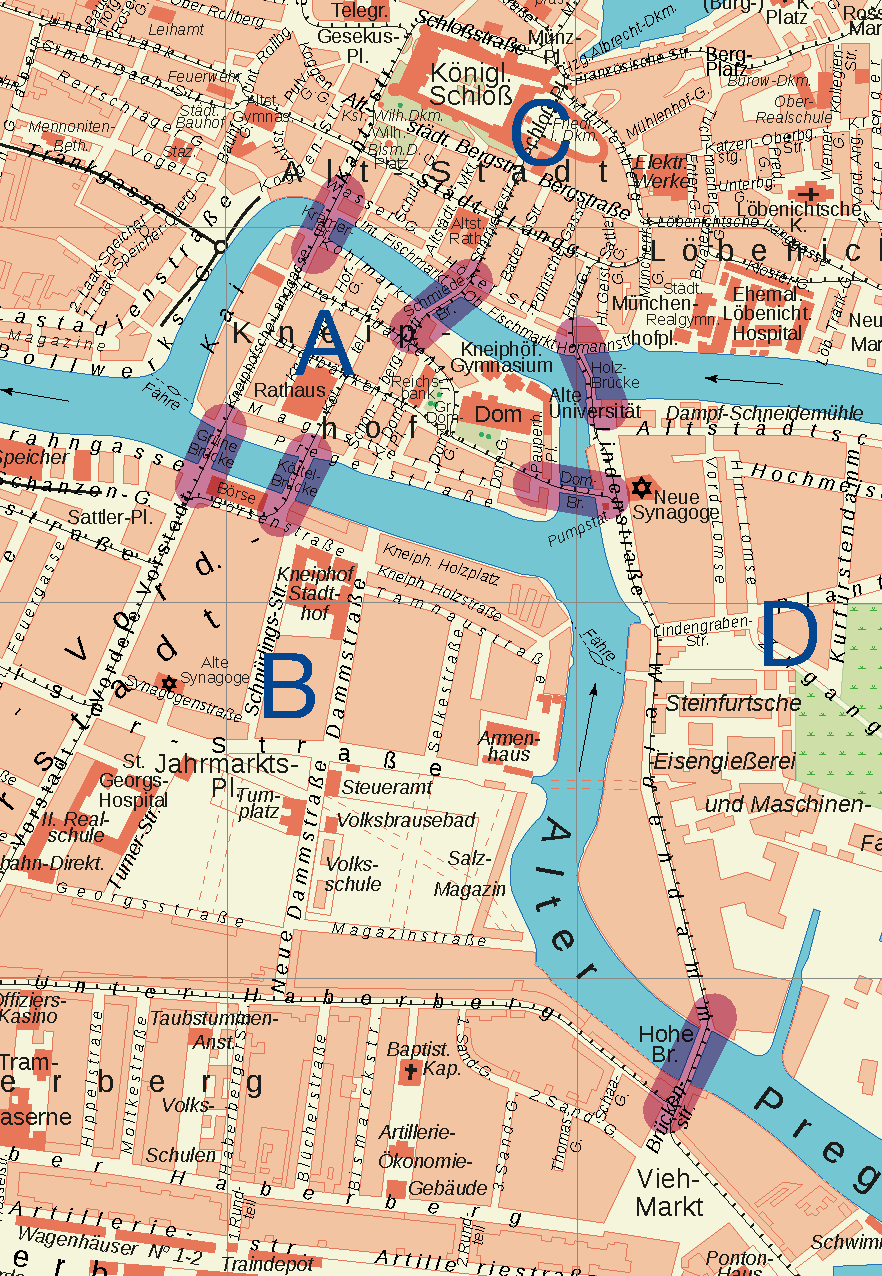
\includegraphics[width=0.5\textwidth]{Grundlagen_Info/02_Graphen/AbstraktionDurchGraphen/Figures/StadplanCropMitBuchstaben.pdf}
\end{figure}
\end{frame}


\begin{frame}[fragile]{Königsberger Brückenproblem}
\begin{itemize}[<+->]
    \item Die vier verschiedenen Stadtteile Kneiphof ($A$), Vorstadt ($B$), Alt-Stadt ($C$) und Lomse ($D$) werden von dem Fluss \textit{Pregel} von einander getrennt.
    \item Die Stadtteile sind durch sieben Brücken verbunden.
\end{itemize}
\end{frame}


\begin{frame}[fragile]{Formulierung des Brückenproblems}
Gibt es einen Weg durch Königsberg, bei dem man alle sieben Brücken \textbf{genau einmal} überquert, und wenn ja, ist auch ein Rundweg möglich, bei dem man wieder zum Ausgangspunkt gelangt?
\end{frame}


% slide 10
\begin{frame}[fragile]{}
\begin{figure}
    \centering
    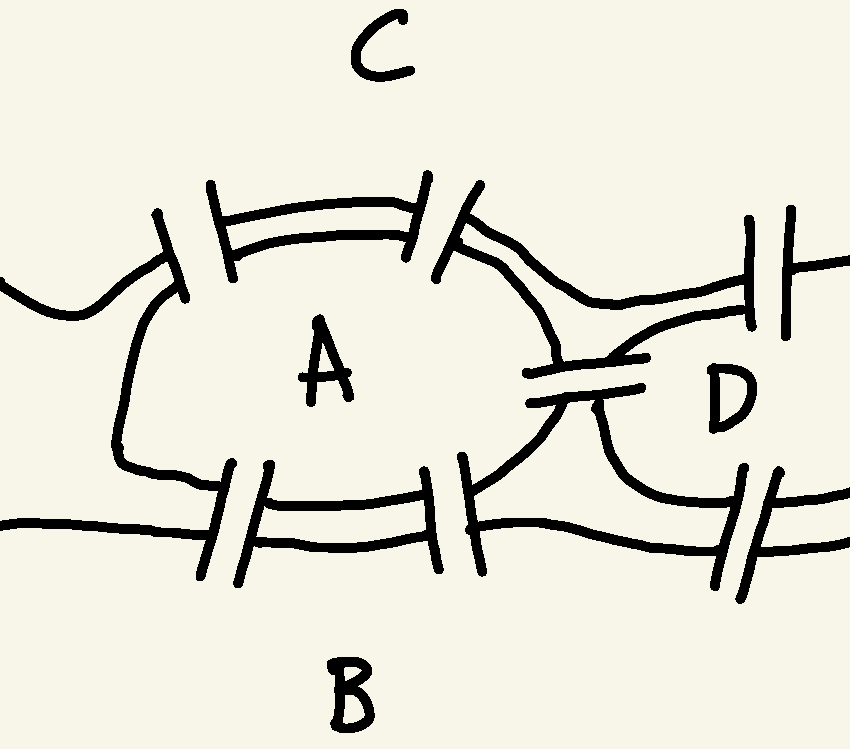
\includegraphics[width=0.9\textwidth]{Grundlagen_Info/02_Graphen/AbstraktionDurchGraphen/Figures/vonHandCrop.pdf}
\end{figure}
\end{frame}


% slide 9
\begin{frame}[fragile]{}
\begin{figure}
    \centering
    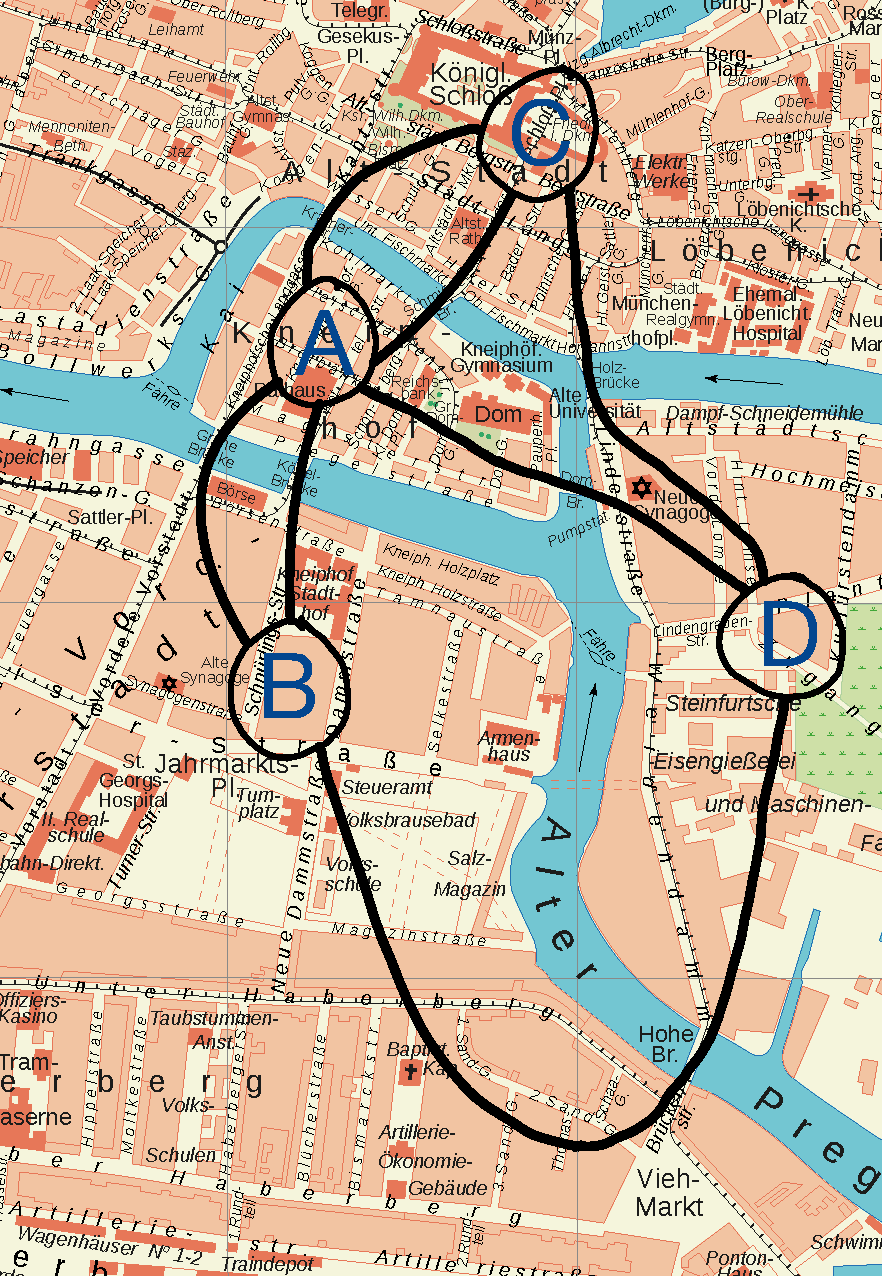
\includegraphics[width=0.5\textwidth]{Grundlagen_Info/02_Graphen/AbstraktionDurchGraphen/Figures/GraphAufStadtplan.pdf}
\end{figure}
\end{frame}

% slide 11
\begin{frame}[fragile]{}
\begin{figure}[H]
\centering
\resizebox{0.3\textwidth}{!}{%
\begin{tikzpicture}[shorten >=1pt,auto,node distance=3cm, semithick, scale=0.1]
  \node[state] (A)              {$A$};
  \node[state] (B) [below of=A] {$B$};
  \node[state] (C) [above of=A] {$C$};
  \node[state] (D) [right of=A] {$D$};

  \path (A) edge [bend right] node[left] {$b_5$} (B)
        (A) edge [bend left] node[left] {$b_6$} (B)
        (A) edge [bend right] node {$b_2$} (C)
        (A) edge [bend left] node {$b_1$} (C)
        (A) edge node {$b_4$} (D)
        (B) edge node[below=5pt] {$b_7$} (D)
        (C) edge node {$b_3$} (D);
\end{tikzpicture}
}%
\caption*{Modellierung des Brückenproblems durch einen Graphen (genauer: Multigraphen)}
\label{fig:Euler}
\end{figure}
\end{frame}


\begin{frame}[fragile]{}
\begin{figure}[H]
\centering
\resizebox{0.3\textwidth}{!}{%
\begin{tikzpicture}[shorten >=1pt,auto,node distance=3cm, semithick, scale=0.1]
  \tikzstyle{every state}=[fill=Red!10,draw=Red,text=black]
  \node[state] (A)              {$\textcolor{Red}{A}$};
  \node[state] (B) [below of=A] {$\textcolor{Red}{B}$};
  \node[state] (C) [above of=A] {$\textcolor{Red}{C}$};
  \node[state] (D) [right of=A] {$\textcolor{Red}{D}$};

  \path (A) edge [bend right,color=Blue] node[left] {$b_5$} (B)
        (A) edge [bend left,color=Blue] node[left] {$b_6$} (B)
        (A) edge [bend right,color=Blue] node {$b_2$} (C)
        (A) edge [bend left,color=Blue] node {$b_1$} (C)
        (A) edge [color=Blue] node {$b_4$} (D)
        (B) edge [color=Blue] node[below=5pt] {$b_7$} (D)
        (C) edge [color=Blue] node {$b_3$} (D);
\end{tikzpicture}
}
\end{figure}
\begin{itemize}[<+->]
    \item Die \enquote{runden Blasen} werden \tib{\textcolor{Red}{Knoten}} genannt. Dieser Graph hat die vier Knoten $A, B, C$ und $D$ (Stadtteile).
    \item Die \enquote{Verbindungslinien} werden \tib{\textcolor{Blue}{Kanten}} genannt. Dieser Graph hat die sieben Kanten $b_1,b_2, \ldots, b_7$ (Brücken).
\end{itemize}
\end{frame}

\begin{frame}[fragile]{}
\begin{figure}[H]
\centering
\resizebox{0.3\textwidth}{!}{%
\begin{tikzpicture}[shorten >=1pt,auto,node distance=3cm, semithick, scale=0.1]
  \tikzstyle{every state}=[fill=Red!10,draw=Red,text=black]
  \node[state] (A)              {$\textcolor{Red}{A}$};
  \node[state] (B) [below of=A] {$\textcolor{Red}{B}$};
  \node[state] (C) [above of=A] {$\textcolor{Red}{C}$};
  \node[state] (D) [right of=A] {$\textcolor{Red}{D}$};

  \path (A) edge [bend right,color=Blue] node[left] {$b_5$} (B)
        (A) edge [bend left,color=Blue] node[left] {$b_6$} (B)
        (A) edge [bend right,color=Blue] node {$b_2$} (C)
        (A) edge [bend left,color=Blue] node {$b_1$} (C)
        (A) edge [color=Blue] node {$b_4$} (D)
        (B) edge [color=Blue] node[below=5pt] {$b_7$} (D)
        (C) edge [color=Blue] node {$b_3$} (D);
\end{tikzpicture}
}
\end{figure}
\begin{itemize}[<+->]
    \item Für einen gegeben Knoten wird die Anzahl der Kanten, welche an diesen Knoten angrenzen, als der \tib{Grad} dieses Knoten bezeichnet.
    \item Der Grad von $A$ in unserem Beispiel ist $5$. Die Grade der Knoten $B, C$ und $D$ sind jeweils $3$.
\end{itemize}
\end{frame}


\begin{frame}[fragile]{Formulierung des Brückenproblems (in der Sprache von Graphen)}
\begin{exampleblock}{Brückenproblem}
Gibt es einen Weg durch Königsberg, bei dem man alle sieben Kanten genau einmal überquert, und wenn ja, ist auch ein Rundweg möglich, bei dem man wieder zum Ausgangspunkt gelangt?
\end{exampleblock}
\end{frame}


\begin{frame}[fragile]{1. Aufgabenblock (5 Minuten, danach kurze Besprechung)}
\begin{center}
    Lösen Sie die beiden Aufgaben 1.1 und 1.2.
\end{center}
\end{frame}

\begin{frame}[fragile]{Lösungsvorschlag zu Aufgabe 1.1}
\begin{itemize}[<+->]
    \item In einem \textbf{sozialen Netzwerk} können die User als Knoten angesehen werden. Dabei sind zwei Knoten genau dann miteinander verbunden, wenn die entsprechenden User miteinander befreundet sind.
    \item In einem \textbf{Modell zur Simulation von Pandemien} können die Menschen als Knoten aufgefasst werden. Dabei sind zwei Knoten genau dann miteinander verbunden, wenn die beiden entsprechenden Menschen in den letzten drei Tagen persönlichen Kontakt zu einander hatten.
\end{itemize}
\end{frame}

\begin{frame}[fragile]{Lösungsvorschlag zu Aufgabe 1.2, Teil (a)}
\begin{figure}[H]
\centering
\begin{tikzpicture}[
node distance = 22mm and 24mm,
every state/.append style = {inner sep=0pt, fill=gray!10,
                             minimum size=11mm},
every edge/.style = {draw, -Triangle, bend angle=15},
                auto=right,
                        ]
\node (L) [state,align=center]        {Lea};
\node (A) [state, above right=of L,align=center]   {Alain};
\node (E) [state, below right=of L,align=center]   {Eldin};
% %
% \draw[gray!30, line width=5pt]
%         (s1) to                     (s2)
%         (s1) to [bend right=15]     (s6);
% %
\draw   (L) edge            (A)
        (L) edge            (E)
        (E) edge             (A);
\end{tikzpicture}
    \caption*{Verlinkung von Webseiten in der Klasse G2B}
\end{figure}
\end{frame}

\begin{frame}[fragile]{Lösungsvorschlag zu Aufgabe 1.2, Teil (b)}
\begin{figure}[H]
\centering
\begin{tikzpicture}[
node distance = 22mm and 24mm,
every state/.append style = {inner sep=0pt, fill=gray!10,
                             minimum size=11mm},
every edge/.style = {draw, -Triangle, bend angle=15},
                auto=right,
                        ]
\node (H) [state,align=center]        {Hendschiken};
\node (W) [state, above right=of L,align=center]   {Wohlen};
\node (E) [state, below right=of L,align=center]   {Effretikon};

\draw   (H) edge [bend right,"5"]           (W)
        (W) edge [bend right,"6"]           (H)
        (E) edge ["56"]            (H)
        (E) edge ["61"]            (W);
\end{tikzpicture}
    \caption*{Zugverbindungen}
\end{figure}
\end{frame}


\begin{frame}[fragile]{2. Aufgabenblock (10 Minuten, ohne Besprechung)}
\begin{center}
    Lösen Sie die drei Aufgaben 1.3, 1.4 und 1.5. Lesen Sie auch die Definition der Eulerwege und Eulerkreise.
\end{center}
\end{frame}


\begin{frame}[fragile]{Beobachtungen zu Eulerkreisen}
\begin{figure}[H]
     \centering
\resizebox{0.4\textwidth}{!}{%
\begin{tikzpicture}[shorten >=1pt,auto,node distance=3cm, semithick, scale=0.1]
  \node[state] (A)              {$A$};
  \node[state] (E) [above right of=A] {$E$};
  \node[state] (B) [below right of=E] {$B$};
  \node[state] (C) [below of=A] {$C$};
  \node[state] (D) [below of=B] {$D$};

  \path (A) edge node {{\tiny $b_1$}} (E)
        (E) edge node {{\tiny $b_2$}} (B)
        (A) edge node {{\tiny $b_3$}} (B)
        (A) edge node {{\tiny $b_4$}} (C)
        (A) edge node[near start, above] {{\tiny $b_5$}} (D)
        (B) edge node[near start, above] {{\tiny $b_6$}} (C)
        (B) edge node {{\tiny $b_7$}} (D);
\end{tikzpicture}
}%
\end{figure}
\noindent
Beispiels eines Eulerkreises in diesem Graphen:
    \begin{align*}
        A \stackrel{b_3}{\longrightarrow} B \stackrel{b_2}{\longrightarrow} E 
        \stackrel{b_1}{\longrightarrow} A \stackrel{b_4}{\longrightarrow}  C \stackrel{b_6}{\longrightarrow} B
        \stackrel{b_7}{\longrightarrow} D \stackrel{b_5}{\longrightarrow} A.
    \end{align*}
\end{frame}


\begin{frame}[fragile]{Notwendige Bedingung für einen Eulerkreis}
\centering
\begin{center}
    (Ein Graph enthält ein Eulerkreis.)
\end{center}
$\Big\Downarrow$\\
\begin{center}
    (Der Grad jedes Knoten in dem Graphen ist gerade.)
\end{center}
\end{frame}


\begin{frame}[fragile]{Begründung}
\begin{align*}
    \textcolor{Blue}{s} \elem{\textcolor{Red}{s\text{ raus}}} v_1 \longrightarrow v_2 \elem{\textcolor{Green}{v_3\text{ rein}}} v_3 \elem{\textcolor{Red}{v_3\text{ raus}}} v_4\longrightarrow v_5\longrightarrow \ldots \longrightarrow v_n \elem{\textcolor{Green}{s\text{ rein}}} \textcolor{Blue}{s}
\end{align*}
\begin{itemize}[<+->]
    \item Jeder Knoten wird genau so oft besucht (rein) wie verlassen (raus)!
    \item Wird ein Knoten also $k$-mal besucht, so wird er auch $k$-mal verlassen. $\Rightarrow$ Es grenzen genau $2k$ (gerade Zahl) Kanten an den Knoten an und somit ist sein Grad eine gerade Zahl!
\end{itemize}
\end{frame}


\begin{frame}[fragile]{3. Aufgabenblock (Rest der Lektion)}
\begin{center}
    Lösen Sie die beiden Aufgaben 1.6 und 1.7.
    
    \noindent
    Falls Sie schon fertig sind: Wenden Sie sich den Aufgaben 1.8 und 1.9 zu.
\end{center}
\end{frame}

\begin{frame}[fragile]{Pause}
\begin{center}
Vielen Dank für Ihre Mitarbeit und Ihre Aufmerksamkeit!
\end{center}
\end{frame}

% \begin{frame}[fragile]{Begründung}
% \begin{align*}
%     \textcolor{Blue}{s} \elem{\textcolor{Red}{s\text{ raus}}} v_1 \longrightarrow v_2 \elem{\textcolor{Green}{v_3\text{ rein}}} v_3 \elem{\textcolor{Red}{v_3\text{ raus}}} v_4\longrightarrow v_5\longrightarrow \ldots \longrightarrow v_n \elem{\textcolor{Green}{s\text{ rein}}} \textcolor{Blue}{s}
% \end{align*}
% \begin{itemize}[<+->]
%     \item Müssen die Knoten $v_1, v_2, \ldots, v_n$ alle verschieden sein?
%     \item Müssen die Kanten (schwarze Pfeile) alle verschieden sein?
%     \item Ist es möglich, dass der Startknoten $\textcolor{Blue}{s}$ auch in der Folge $v_1, v_2, \ldots, v_n$ (nicht nur am Anfang und Ende) vorkommt?
% \end{itemize}
% \end{frame}


% \begin{frame}[fragile]{Begründung}
% \begin{itemize}[<+->]
%     \item Angenommen in einem Graphen existiert ein Eulerkreis. Lassen Sie uns diesen Eulerkreis gedanklich zeichnen.
%     \item Mit dem Zeichnen werden wir bei einem Knoten $s$ beginnen und schliesslich den Kreis in diesem Knoten beenden.
% \end{itemize}
% \end{frame}

% \begin{frame}[fragile]{Begründung}
% \begin{itemize}[<+->]
%     \item Betrachten wir aber zuerst einen beliebigen Knoten $v$, der nicht unser Startknoten $s$ ist.
%     \item Es kann sein, dass wir $v$ beim Zeichnen des Eulerkreises mehrmals (mindestens einmal) besuchen.
%     \item Da wir den Kreis nicht in $v$ (sondern $s$) beenden, kann $v$ keine Sackgasse sein. Somit müssen wir jedes Mal, wenn wir in $v$ hinein gehen, $v$ auch wieder verlassen.
%     \item Da wir keine Kante mehrmals verwenden dürfen, verwenden wir dabei jedes mal eine neue Kante. 
%     \item Die Gesamtzahl der an $v$ angrenzenden Kanten ist also doppelte so gross wie die Anzahl unserer Besuche von $v$ und somit gerade.
% \end{itemize}
% \end{frame}


% \begin{frame}[fragile]{Begründung}
% \begin{itemize}[<+->]
%     \item Wie steht es um den Startknoten $s$?
%     \item Wir verlassen $s$ zu Beginn über eine Kante.
%     \item Danach kann $s$ mehrmals besucht werden, bevor wir den Kreis abschliessen. Doch jeder dieser zwischenzeitlichen Besuche von $s$ verwendet genau 2 Kanten (eine hin zu $s$ und eine weg von $s$).
%     \item Am Ende wird $s$ ein letztes Mal besucht und der Eulerkreis endet bei $s$. Zusammen mit der Kante für das anfängliche Verlassen (hinaus) und den finalen Besuch (hinein), grenzt also auch eine gerade Zahl von Kanten an $s$ an.
% \end{itemize}
% \end{frame}